\section{Techniques}

  \subsection{ENet\cite{paszke2016enet}}

    \ti{Efficient Neural Network} (ENet) is a \tb{lightweight} neural network designed
    for \tb{real-time} semantic segmentation. It is based on a deep residual network (ResNet)
    with a modified architecture. The main idea is to reduce the number of parameters and
    operations while maintaining the accuracy of the network\cite{paszke2016enet}.
    
    \subsubsection{Architecture}

      \paragraph{Initial Block}

        The initial block is a \ti{convolutional layer} with a \ti{stride of 2}
        and a \ti{kernel size of 3}. It is used to reduce the size of the input image
        by a factor of 2. The number of output channels is 16\cite{paszke2016enet}.
        This block perfomrs initial feature extraction and dimensionality reduction,
        as shown in figure \ref{fig:enet_initial_block}.
        \begin{figure}[htbp]
          \centering
          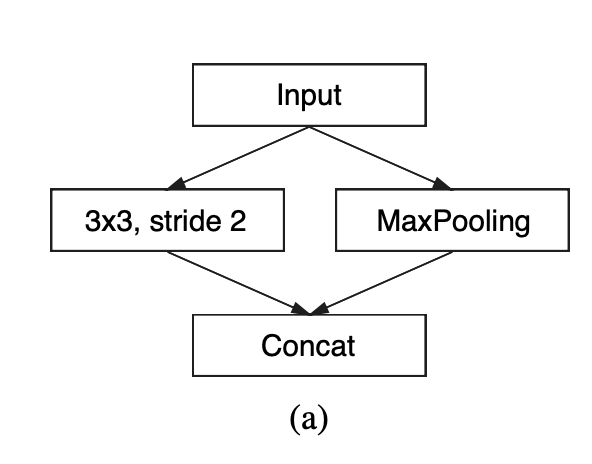
\includegraphics[width=0.60\linewidth]{techniques/enet_initial_block.png}
          \caption{ENet initial block\cite{paszke2016enet}}
          \label{fig:enet_initial_block}
        \end{figure}

      \paragraph{Bottleneck}

        The bottleneck block is a sequence of layers including \ti{1x1 convolution},
        \ti{3x3 convolution} and \ti{1x1 convolution} in this order. The first
        \ti{1x1 convolution} is used to reduce the number of input channels,
        the \ti{3x3 convolution} is used to extract features and the second
        \ti{1x1 convolution} is used to increase the number of output channels.
        5x5 convolution decomposed into two asymmetric ones\cite{paszke2016enet},
        as shown in figure \ref{fig:enet_bottleneck}.
        \begin{figure}[htbp]
          \centering
          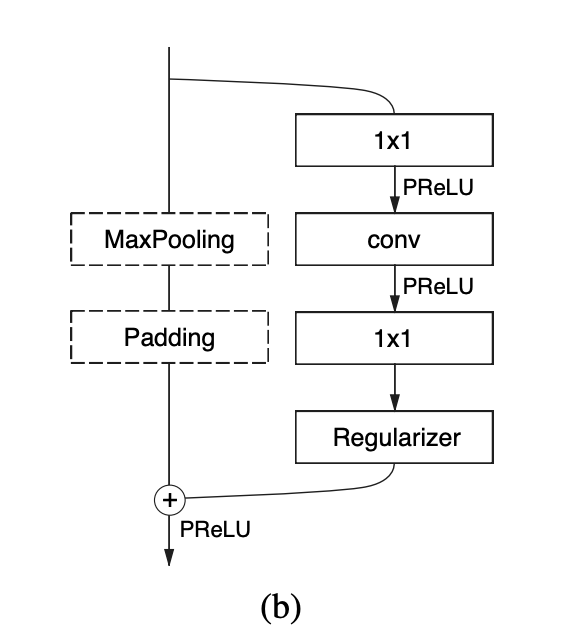
\includegraphics[width=0.60\linewidth]{techniques/enet_bottleneck.png}
          \caption{ENet bottleneck\cite{paszke2016enet}}
          \label{fig:enet_bottleneck}
        \end{figure}

  \subsection{ESPNet\cite{mehta2018espnet}}

    \ti{Efficient Spatial Pyramid Network} (ESPNet) is based on a new convolutional
    layer called \ti{efficient spatial pyramid convolution} (ESPConv), based on a
    convolutional factorization principle that decompose a standard convolution
    into a set of smaller convolutions\cite{mehta2018espnet}. ESPConv is divided
    into two steps: \ti{point-wise convolution} and \ti{spatial pyramid of dilated
    convolutions}. The point-wise convolution is used to reduce the number of
    input channels, while the spatial pyramid of dilated convolutions re-samples
    the input feature map at different scales. The ESPConv is shown in figure
    \ref{fig:espnet_espconv}.
    \begin{figure}[htbp]
      \centering
      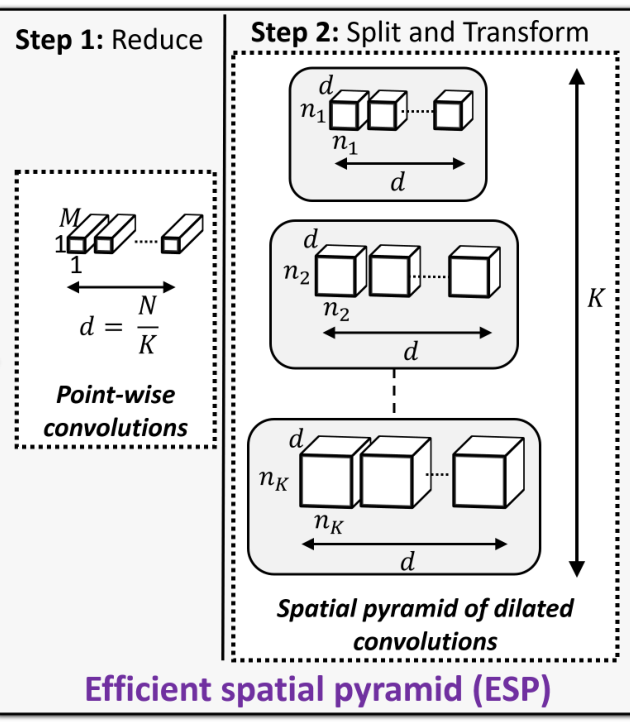
\includegraphics[width=0.60\linewidth]{techniques/espnet_espconv.png}
      \caption{ESPConv\cite{mehta2018espnet}}
      \label{fig:espnet_espconv}
    \end{figure}
    ESPNEt uses ESPConv to replace the standard convolution kernels, as well as 
    down-sampling operations, except for the first convolutional layer which is
    a standard convolutional\cite{mehta2018espnet}. All ESPConv layers are
    followed by a batch normalization layer and a PReLU activation function.
    Finally, the last layer feeds the output to a softmax function to obtain
    the probability of each class\cite{mehta2018espnet}.

  \subsection{FPN\cite{lin2017feature}}

    \ti{Feature Pyramid Network} (FPN) is a feature extraction architecture
    that combines low-resolution, semantically strong features with high-resolution,
    semantically weak features via a top-down pathway and lateral connections\cite{lin2017feature}.
    The FPN is shown in figure \ref{fig:fpn}.
    \begin{figure}[htbp]
      \centering
      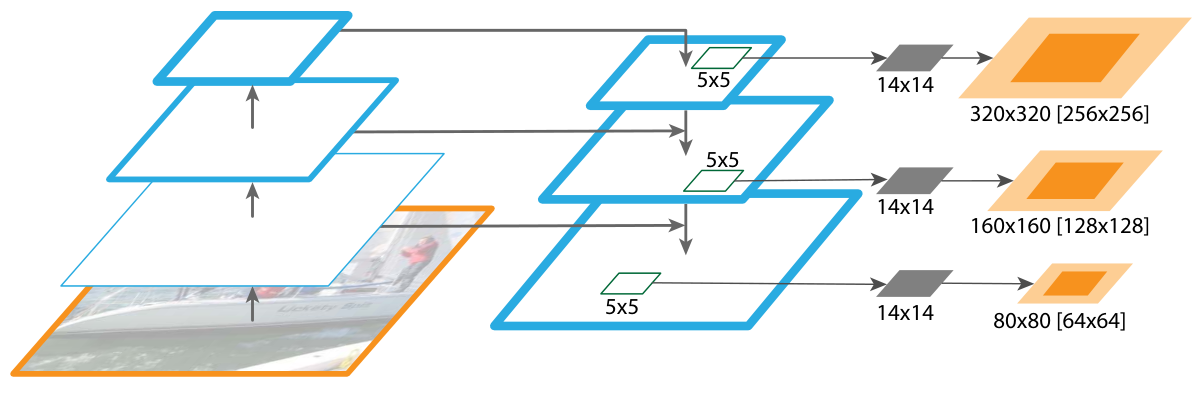
\includegraphics[width=0.60\linewidth]{techniques/fpn.png}
      \caption{FPN\cite{lin2017feature}}
      \label{fig:fpn}
    \end{figure}
    FPN leverage the inherent multi-scale, pyramidal hierarchy of deep convolutional
    networks to construct feature pyramids with marginal extra cost. The feature
    pyramids are used for object detection and semantic segmentation\cite{lin2017feature}.

    \subsubsection{Architecture}

      \paragraph{Bottom-up Pathway}

        The bottom-up pathway is the usual feed-forward computation in a convolutional
        network. It is used to compute a feature hierarchy consisting of feature maps
        at different scales with strong semantics\cite{lin2017feature}. FP define a
        pyramid level for each stage, and choose the last layer of each stage as the
        output of that level since it has the strongest semantics\cite{lin2017feature}.

      \paragraph{Top-down Pathway and Lateral Connections}

        The top-down pathway is used to generate high-resolution feature maps by upsampling
        the coarse feature maps. The lateral connections are used to fuse the high-resolution
        features with the low-resolution features\cite{lin2017feature}.
